\documentclass[letterpaper, 10pt]{article}
%\usepackage{palatino}
\usepackage{hyperref}
\usepackage{graphicx}
\renewcommand{\baselinestretch}{1.2}
\usepackage[margin=1.2in]{geometry}

\begin{document}
\title{WebPlotDigitizer User Manual\\ Version 2.6}
\author{Ankit Rohatgi\footnote{E-Mail: ankitrohatgi@hotmail.com}}
\maketitle
\tableofcontents
\newpage
\section{Introduction}
A large quantity of useful data is available only in graphical form as plots in images. In these images, it is easy to determine the relationship between the variables involved, but recovering the exact numerical values of the data is usually a tedious and error prone process. To aid this time consuming task of data recovery, several digitization softwares have been developed over the years. However, even with the abundance of free and commercial softwares, this task remains daunting and prone to errors. Many of the existing softwares are either designed to work only on specific operating systems or work with a limited variety of plots. Some are just difficult to use or prone to errors. Finally, many require a paid license which prevents their widespread use by students, independent researchers or organizations with limited resources.

Because of the above limitations in current digitizing softwares, WebPlotDigitizer was developed to facilitate easy and accurate data extraction from a variety of plot types and also maps. This program has been built using HTML5 which allows it to run within most popular web browsers and does not require an installation process that is performed by the user.

\begin{figure}
\begin{center}
\includegraphics[width=6in]{./figures/screenshot.png}
\caption{Screenshot of WebPlotDigitizer showing the data points recovered on a plot via automatic detection.}
\end{center}
\end{figure}

\subsection{History}
WebPlotDigitizer was initially developed while working on my graduate studies at the University of Notre Dame. Having to pull out data from several publications for comparing and contrasting my own findings in the lab was too painful even for someone studying fluid-particle interactions in suspensions flowing at low Reynolds numbers. The search for a tool to aid this process usually ended in realizing that most of the existing softwares for this purpose did not fulfill many of the requirements. I was faced with a similar task as an undergraduate student. Back then, just writing a simple Java based code for picking a few points by clicking on them manually was sufficient. My advisor at Notre Dame also had a Matlab code to do this job for two dimensional XY plots, but the points still had to be picked manually. Both the options were not very convenient.

Some of the experimental work in the lab required me to learn some basic image processing techniques which eventually formed the basis of the automatic detection algorithms used here. Image processing knowledge along with some interest in learning the much publicized HTML5 APIs at the time were a perfect match to create a web based data extraction tool like this.

Considering the significant interest in this software, I have continued to refine the software in my spare time even after completing my graduate studies in 2012.
\subsection{User Manual}
This user manual describes the various capabilities of the software and aims to help the user in making an effective use of the software. 
\\
\\
This manual is available online at \url{http://arohatgi.info/WebPlotDigitizer} in PDF or HTML format.

\subsection{Other Resources}
While other resources to find technical information about the software are being put together, some video tutorials by the author are available at \url{http://arohatgi.info/WebPlotDigitizer}.

\subsection{License}
WebPlotDigitizer is distributed under GNU General Public License version 3 by Ankit Rohatgi. For complete terms and conditions, please refer to \url{http://www.gnu.org/copyleft/gpl.html}
\subsection{Source Code}
WebPlotDigitizer is an open source software available under GNU General Public License version 3. The source code can be obtained from GitHub (\url{https://github.com/ankitrohatgi/WebPlotDigitizer/}). Please contact me via email if you wish to contribute to this project.

\subsection{Availability}
The latest released version of the software can be used directly from the website \url{http://arohatgi.info/WebPlotDigitizer}. For the Google Chrome web browser, an \emph{app} pointing to the online software is also available at the Chrome App Store (\url{https://chrome.google.com/webstore/category/apps}).

\subsection{Supported Browsers}
Version 2.6 was ensured to work without major issues on the following browsers:
\begin{itemize}
\item{Safari 6.0.5 on Mac OS 10.8.5}
\item{Google Chrome on Max OS 10.8.5}
\item{Firefox on Windows 7 32-bit}
\item{Internet Explorer 10 on Windows 7 32-bit}
\item{Firefox on Xubuntu Linux}
\end{itemize}
It is expected that browsers similar in functionality and support for the HTML5 API should not have any major problems executing the version 2.6.

\subsection{Citing WebPlotDigitizer}
If you wish to cite WebPlotDigitizer in any of your works, then please use the following information:

\begin{center}
\begin{tabular}{|r|l|}
\hline
Author & Ankit Rohatgi\\
Title & WebPlotDigitizer\\
Website & \url{http://arohatgi.info/WebPlotDigitizer}\\
Version & 2.6\\
Date & October, 2013\\
E-Mail & ankitrohatgi@hotmail.com\\
\hline
\end{tabular}
\end{center}


\subsection{Reporting Issues}
In case of issues with the data recovery, access to the software or general technical questions, feel free to contact the author, Ankit Rohatgi via E-Mail: ankitrohatgi@hotmail.com
\\
\\
Issues specific to bugs in the software can be reported on the issues page on GitHub: \url{https://github.com/ankitrohatgi/WebPlotDigitizer/issues}

\subsection{Future Goals}

\section{Loading Plots}
The image file containing the figure to be analyzed can be loaded into the software in the following ways:
\begin{enumerate}
\item{{\bf Drag \& Drop Operation:} Click down on the file icon in the file browser and move the mouse over the area containing the previous image in WebPlotDigitizer. Release the mouse button to load the file in the software.}
\item{{\bf Browse File on Hard Drive:} Click on the \emph{Load File} button on the top left of WebPlotDigitizer. A popup should show up with a control labelled \emph{Choose File}. Use this control to look for the desired file.}
\item{{\bf Copy-Paste from Clipboard:} This is only supported in Google Chrome web browser. An image selected by copying in a PDF or an image viewer can be pasted on to the software via a simple copy-paste operation.}
\end{enumerate}

\subsection{Supported Image Formats}
WebPlotDigitizer relies on the image formats supported by the HTML5 \emph{canvas} element. Most browsers support common image formats such as JPEG, PNG, BMP and GIF. Since the support for an image format depends on the browser used with the software, please refer to your browser's manual for details. For popular browsers, you can also refer to Wikipedia (\url{http://en.wikipedia.org/wiki/Comparison_of_web_browsers#Image_format_support}).




\section{Edit Image}

\begin{figure}
\begin{center}

\includegraphics[width=3in]{./figures/topButtons.png}
\caption{The top row of buttons in WebPlotDigitizer.}
\label{fig:topButtons}
\end{center}
\end{figure}

If the loaded image needs to be inverted or if only a small area of the image is relevant, then you may wish to use some of the editing tools available by clicking the \emph{Edit Image} button in the top toolbar (Figure \ref{fig:topButtons}). Clicking this button will make a set of buttons appear in the sidebar as shown in Figure \ref{fig:imageEditingSidebar}. The buttons available here are for the following purpose:
\begin{enumerate}
\item{{\bf H. Flip:} Invert the image horizontally.}
\item{{\bf V. Flip:} Invert the image vertically.}
\item{{\bf Crop:} Crop a rectangular region from the image. The user can draw the desired rectangular region on the image after clicking this button.}
\item{{\bf Restore: } Restores the originally loaded image.}
\item{{\bf Save .PNG:} Opens a new tab containing the edited image.}
 
\end{enumerate}




\begin{figure}
\begin{center}
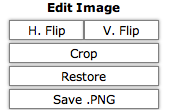
\includegraphics[width=1.5in]{./figures/imageEditingSidebar.png}
\caption{A few basic tools for editing the loaded image are available.}
\label{fig:imageEditingSidebar}
\end{center}
\end{figure}


\section{Define Axes}

After editing the image as needed (or not at all),  you should define the axes used in the plot. This step is required for the software to correctly map the image pixels to possible data points in the image. Depending on the plot type, you will have to select a few known points on the axes. On clicking the \emph{Define Axes} button (see Figure \ref{fig:topButtons}), you should be presented with the menu shown in Figure \ref{fig:defineAxesPopup}.
\begin{figure}
\begin{center}
\includegraphics[width=3in]{./figures/defineAxesPopup.png}
\caption{Popup with plot types that are supported in the software.}
\label{fig:defineAxesPopup}
\end{center}
\end{figure}

\subsection{2D (X-Y) Plot}
Most plots that are on a two dimensional cartesian coordinate system fall under this category. Two dimensional plots that are skewed such that the axes are not mutually perpendicular will also work. Also, neither the horizontal or the vertical axes need to be perfectly aligned with the horizontal and vertical lines of the computer. An image rotated by an angle should also work. 

On selecting this option, you should be presented with popup which asks you to click on two points on the horizontal axis and two on the vertical axis. After clicking \emph{Proceed} on that popup, click on two points on one of the two axes $(x_1, x_2)$ and two on the other $(y_1, y_2)$. For better accuracy during the digitization process, pick the points that are as far away from each other as possible. Also, remember the values on the axes of the points as you will be required to enter those once four points have been clicked on.

After the four points that are required have been clicked on, a popup will appear where you will be required to enter the values at these points. This helps the software map the image pixels corresponding to data points to their actual values when the image is digitized.

\begin{figure}
\begin{center}
\includegraphics[width=2in]{./figures/xyAxesInfo.png}
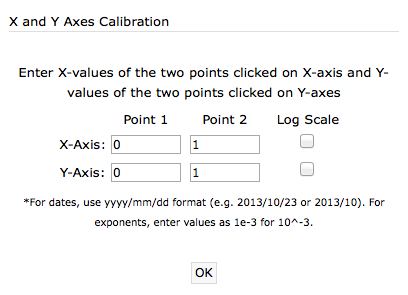
\includegraphics[width=3in]{./figures/xyAlignment.png}
\caption{Alignment for 2D (X-Y) Plot.}
\label{fig:xyAlignment}
\end{center}
\end{figure}

\subsubsection{Format of Calibration Values}
Like most computer programs, WebPlotDigitizer accepts integers (e.g. 1, 2, 3 etc.) or floating point numbers (e.g. 3.14159). However, some extra things to keep in mind are as follows:
\begin{enumerate}
\item{Fractions (e.g. $1/2$) are not computed as numbers.}
\item{For exponentials, the caret symbol (\^{}) is not recognized and the values have to be entered as 1.45e-10 for $1.45 \times 10^{-10}$ (for example).}
\item{{\bf Dates:} This is enabled only for 2D (X-Y) Plots. At the time of calibration, the dates have to be entered in the format shown below. However, with the final digitized data, results can be formatted in many different ways (see section X).
\begin{center}
\begin{tabular}{|c|c|c|}
\hline
Date & Format & Examples\\
\hline
Year, Month and Date & YYYY/MM/DD & 2012/10/23, 2012/10/5 or 2012/10/05\\
Year, Month & YYYY/MM & 2012/10 or 1989/5\\
Year & YYYY & 2012 (treated as any integer)\\
\hline
\end{tabular}
\end{center}
}
\end{enumerate}





\subsection{Polar Diagram}
\subsection{Ternary Diagram}
\subsection{Map With Scale Bar}
\subsection{Image (Align to image pixels)}
\subsection{Workarounds}


\section{Data Acquisition}
\subsection{Manual Mode}
\subsection{Automatic Mode}
\subsubsection{Foreground Color (FG)}
\subsubsection{Background Color (BG)}
\subsubsection{Mark Region}
\subsection{Digitization Algorithms}
\section{CSV Data}

\section{Examples}
\end{document}
